\documentclass{mylib/reporteConCalif}
\title{Reporte}
\author{rodrigofranciscopablo }

\subject{Laboratorio de Diseño Digital}
\mytitle{Reporte de práctica 3}
\mysubTitle{Funciones Lógicas}
\students{Francisco Pablo \textsc{Rodrigo}}
\teacher{M.I. Guevara Rodríguez \textsc{Ma. del Socorro}}
\group{6}
\deliverDate{4 de marzo de 2019}

\newcommand{\funx}{x_1(a,b,c,d) = [a \cdot \overline{b}(c+b \cdot d) + \overline{a} \cdot \overline{b} ]c}

\begin{document}

\coverPage

\tableofcontents
\newpage

\section{Objetivos}

\subsection{General}

El alumno analizará las matemáticas lógicas que sustentan al diseño digital y representará las operaciones lógicas con compuertas.

\subsection{Particular}

El alumno analizará, diseñará e implementará funciones algebraicas por medio de la minimización Booleana, utilizando compuertas básicas.

\section{Introducción}

Es una rama especial del álgebra que se usa principalmente en electrónica digital. El álgebra booleana fue inventada en el año 1854 por el matemático inglés George Boole.
El álgebra de Boole es un método para simplificar los circuitos lógicos (o a veces llamados circuitos de conmutación lógica) en electrónica digital.
El Álgebra de Boole es un sistema matemático que utiliza variables y operadores lógicos. Las variables pueden valer 0 o 1. Y las operaciones básicas son OR(+) y AND(·). Luego se definen las expresiones de conmutación como un número finito de variables y constantes, relacionadas mediante los operadores (AND y OR).
Existen un par de leyes fundamentales que rigen el álgebra de Boole las cuales se enuncian a continuación.\\

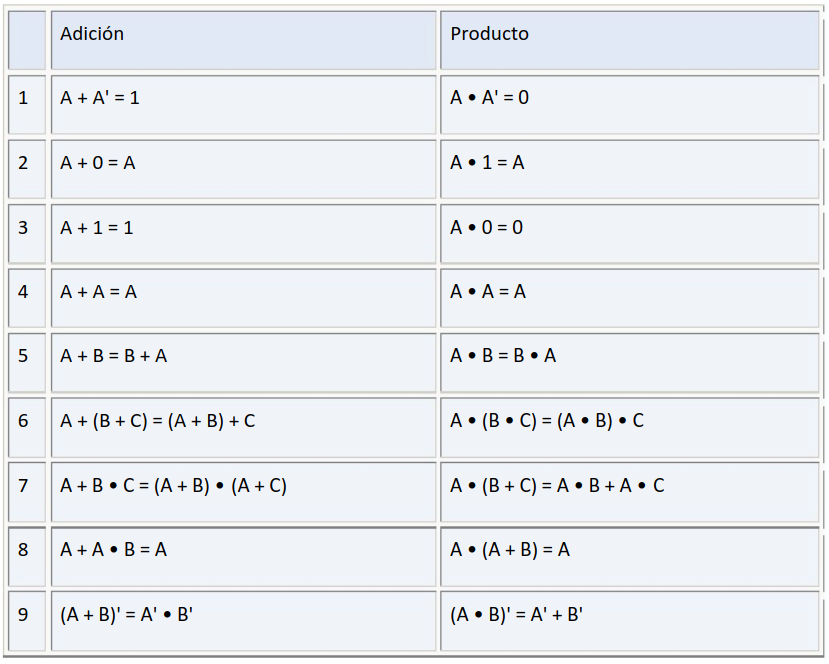
\includegraphics[width=8cm]{img/labdise_practica3/image9}

\newpage
\section{Previo}

\newpage
\section{Desarrollo}

Para el desarrollo de esta práctica construimos la funcion booleana $\funx$ en un diagrama esquemático de \textit{Xilinx} como se muestra acontinuación.\\

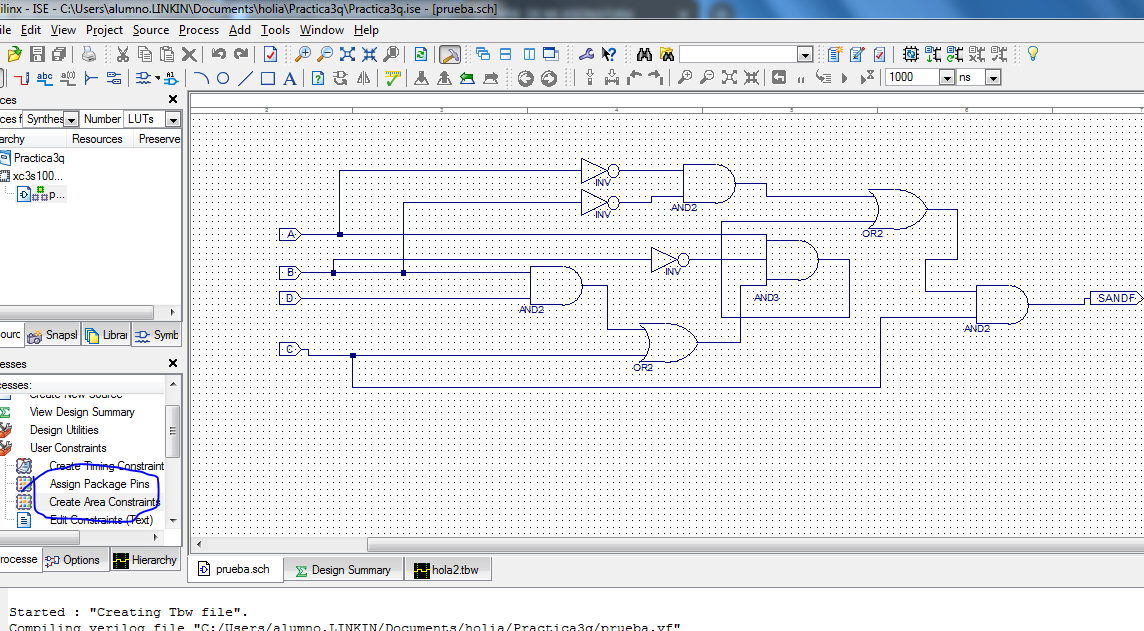
\includegraphics[width=15cm]{img/labdise_practica3/image10}\\

Luego debemos sintetizar nuestro programa para asegurarnos de que no haya errores y que las salidas sean efectivamente las que esperamos para lo cual recurrimos a la ventana que nos muestra un tren de pulsos como se observa a continuación.\\

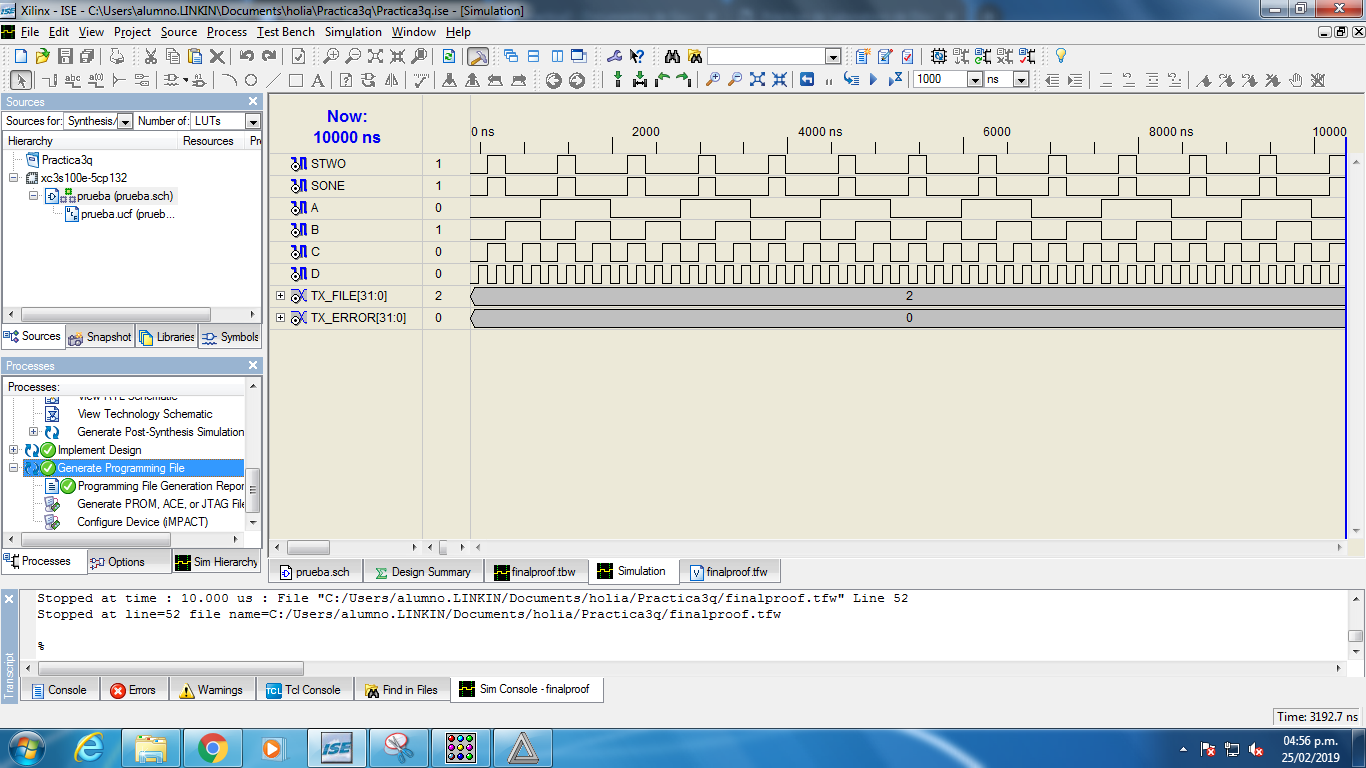
\includegraphics[width=15cm]{img/labdise_practica3/image4}\\

Una vez que nuestro diseño fue realizado correctamente procedemos a descargar el programa en la FPGA, para ello debemos indicarle al programa que queremos utilizar un \textit{Area Constraints} y en la ventana que se abrirá ligaremos los pines que vamos a usar del la FPGA con nuestro diseño.\\

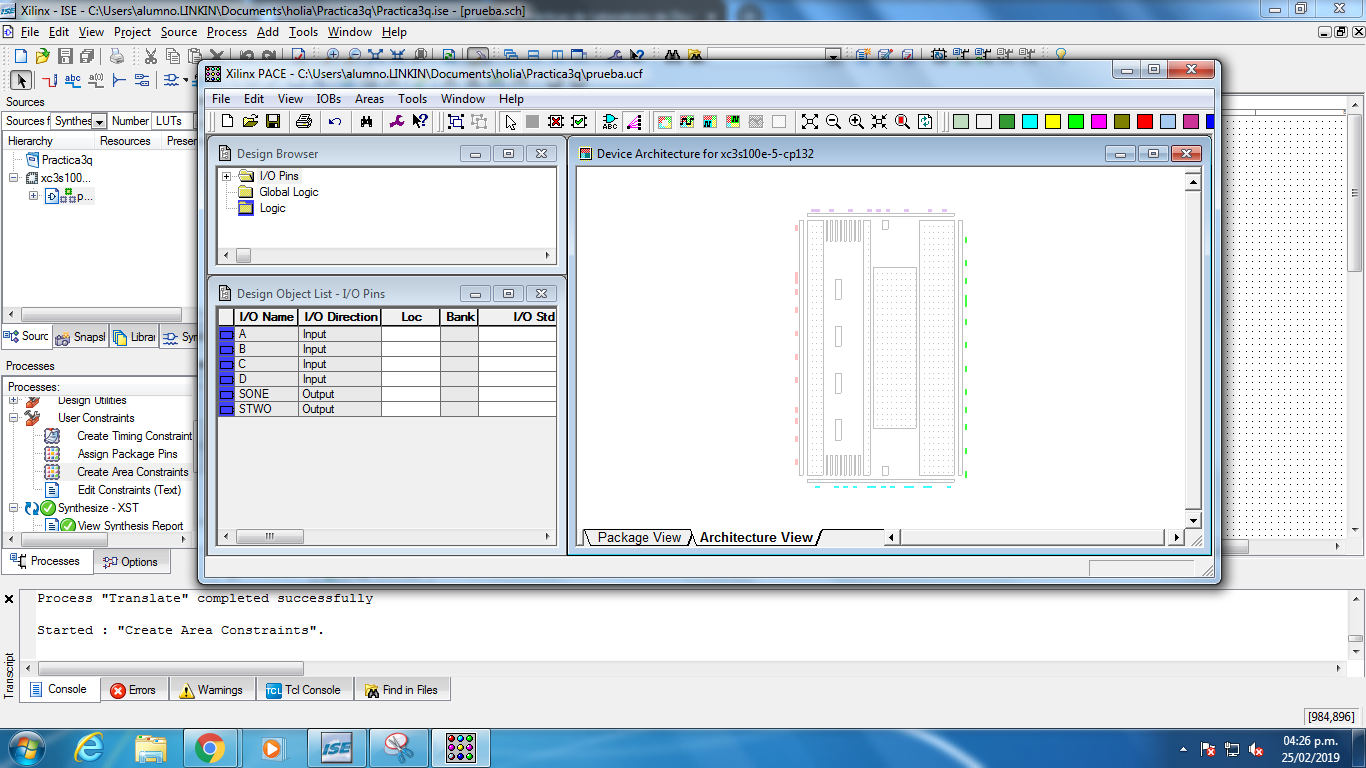
\includegraphics[width=15cm]{img/labdise_practica3/image7}\\

Finalmente para cargar el diseño a la FPGA, en nuestro caso utilizaremos la \textit{Basys o Spartan3E} para lo cual abriremos un programa llamado \textit{ADEPT} \\

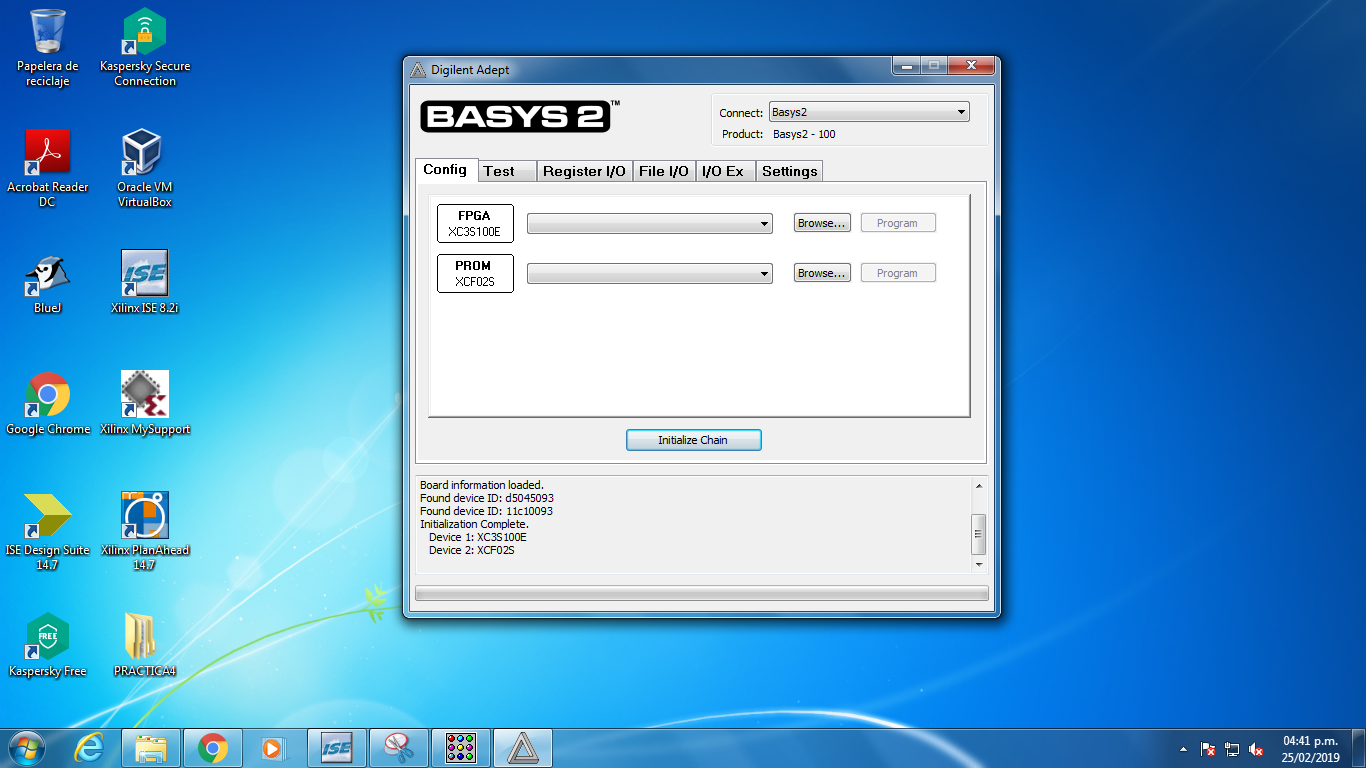
\includegraphics[width=15cm]{img/labdise_practica3/image5}\\

Conectamos la FPGA a nuestra computadora y verificamos que el programa la reconozca. \\

Finalmente debemos buscar el archivo que le cargaremos, dicho archivo fue producido por nuestro programa Xilinx y tiene extensión .bit. Una vez que lo encontremos los seleccionamos y cargamos dicho programa a la tarjeta.\\

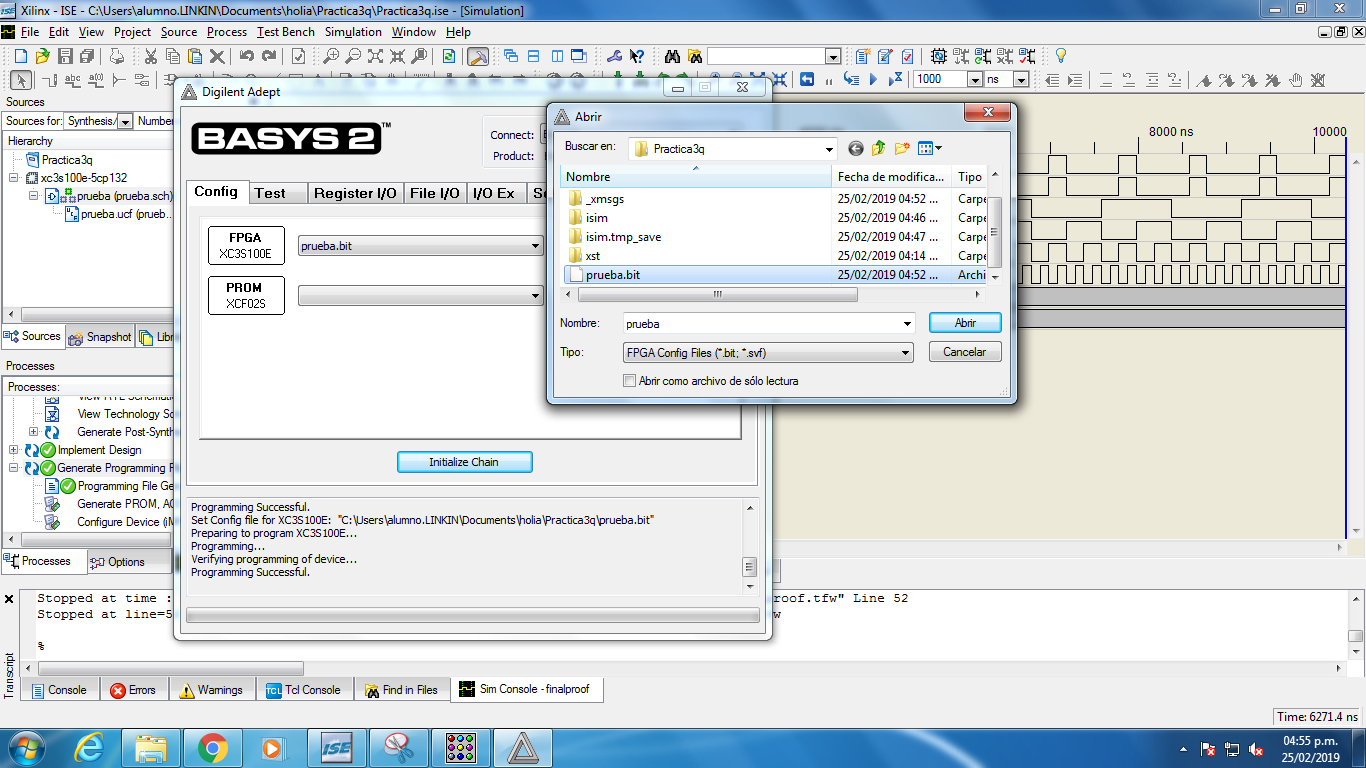
\includegraphics[width=15cm]{img/labdise_practica3/image1}\\

Ahora tenemos nuestro primer programa cargado en la FPGA y puede verse como tiene dos LEDS encendidos que también podrían estar apagados de acuerdo a la configuración de los switches de abajo.\\

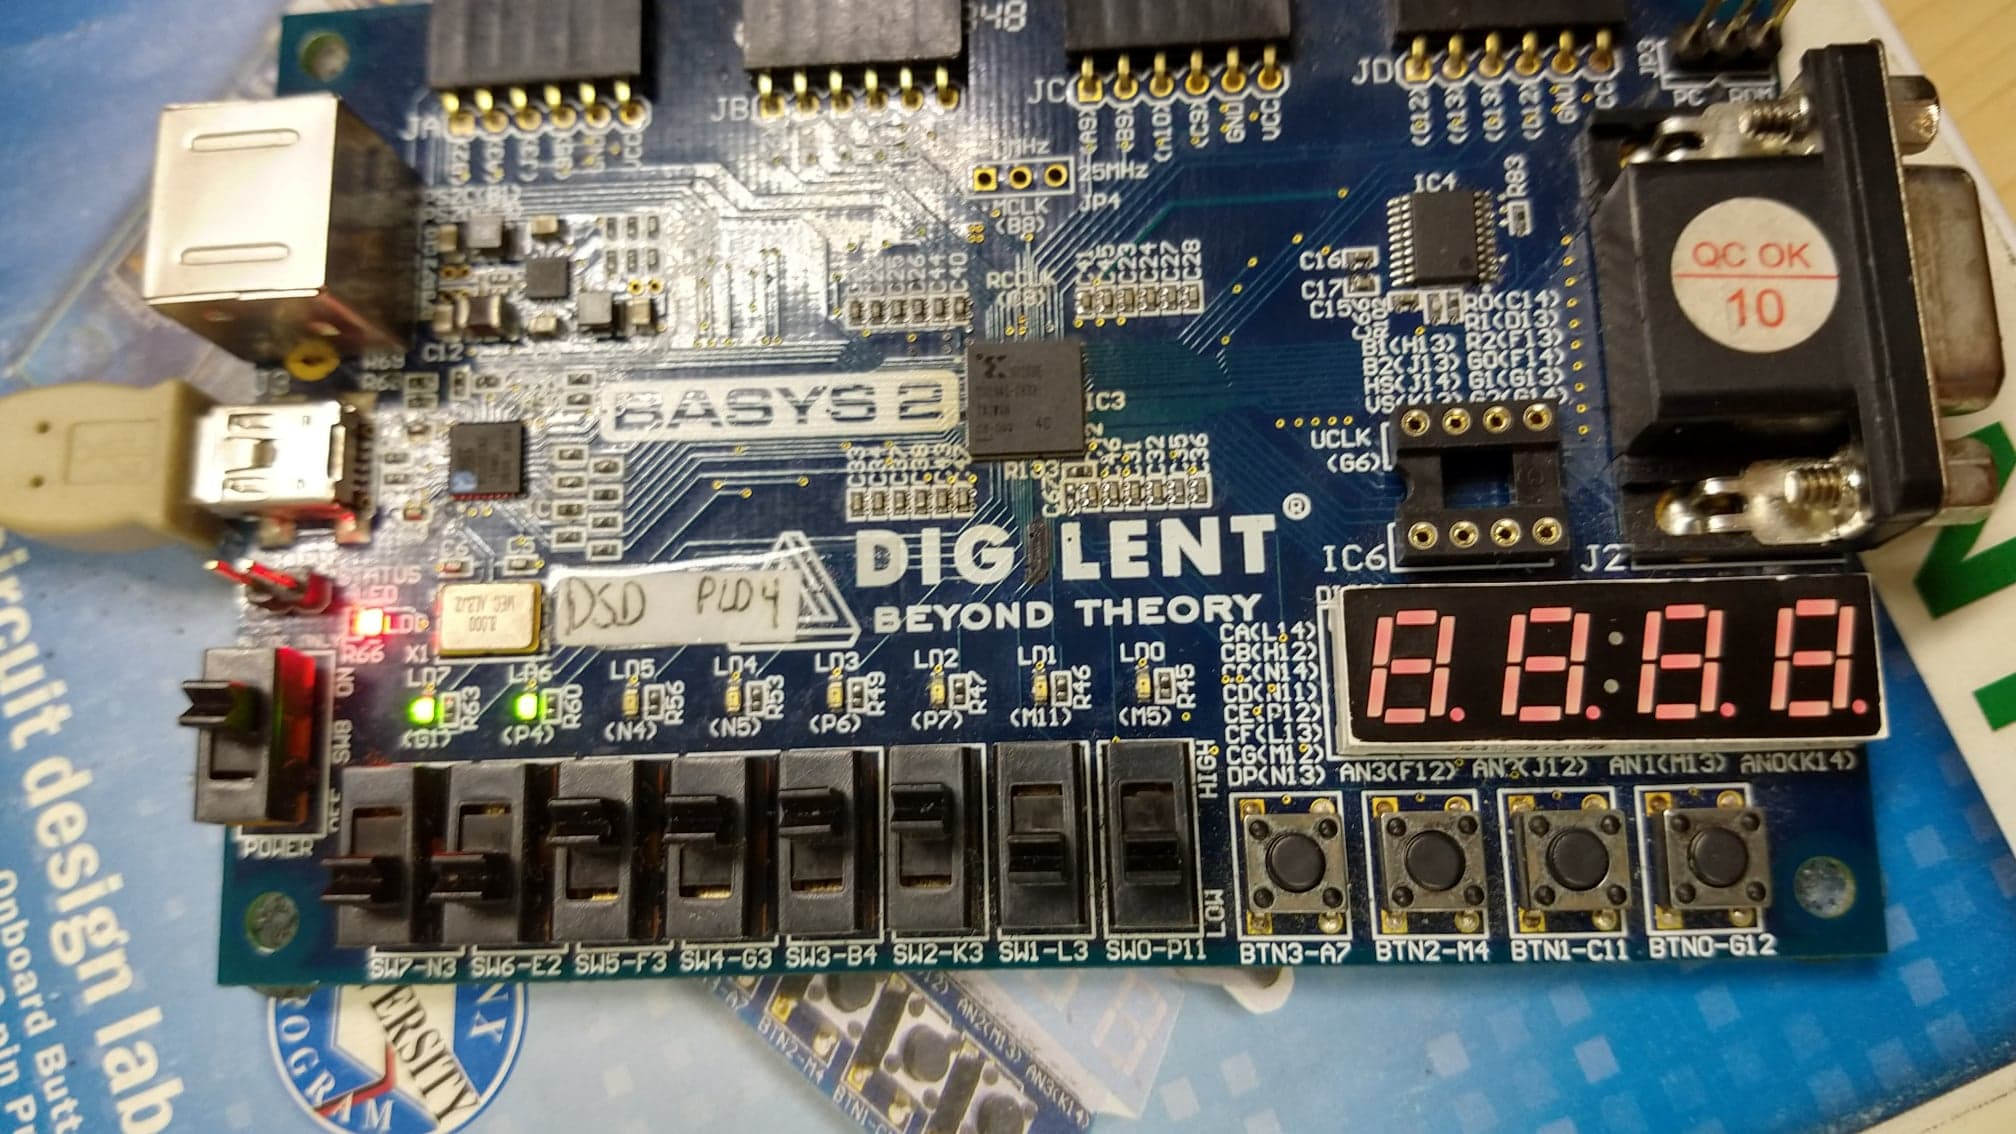
\includegraphics[width=15cm]{img/labdise_practica3/funciona}\\

\section{Conclusiones}

Tener una FPGA hace que solo nos preocupemos por el desarrollo de nuestro circuito ya que si no la tuvieramos tendríamos que tener algunos circuitos integrados (compuertas AND y OR), alambre, botones, LEDs y alguna que otra resistencia. Además de que el tiempo de armado sería como alrededor de dos o tres horas, en cambio con la tajeta que ya tiene todo integrado nos tardadamos como media hora y eso considerando que somos usuarios que apenas estan aprendiendo a usarla.\\

Finalmente esta práctica ayudo a entender de manera más puntual como es que funciona el Algebra de Boole y su relación con la electrónica. Al inicio de la práctica ya sabíamos hacer álgebra de Boole sin embargo no entendiamos del todo bien como aplicarla, después de la práctica nos damos cuenta de su importancia en el mundo electrónico.

\end{document}